% !TEX root = ./physics_of_fluids.tex
% !TEX TS-program = xelatex
% !TEX encoding = UTF-8 Unicode
\chapter{Boundary conditions and interfaces}
\label{chap:boundary_conditions}
We have seen in the previous chapter how to express mass and momentum conservation at the fluid particle level, and we have derived the corresponding equations for fluid motion. These equations are naturally associated with \textbf{boundary conditions} that either express conservation laws (e.g. no mass flux at a boundary) or peculiar physical processes occurring at a surface (temperature or velocity continuity). In both cases these boundary conditions will be pivoting in the determination of the solution.

One striking experimental demonstration of this coupling between the large and the small is provided Fig.~\ref{fig:splash_no_splash}, where two seemingly identical spheres impacting water at the same speed either enter the pool very smoothly or by creating a considerable splash. Actually the difference between the two spheres is a nanometre-thick coating making the sphere either hydrophilic or hydrophobic\index{boundary conditions!hydrophobic, hydrophilic}, thereby revealing how nanometric effects at the boundary can influence large-scale hydrodynamics \citep{Duez2007,Eggers2007}.
\setlength{\unitlength}{1cm}
\begin{figure}[htbp]
\begin{center}
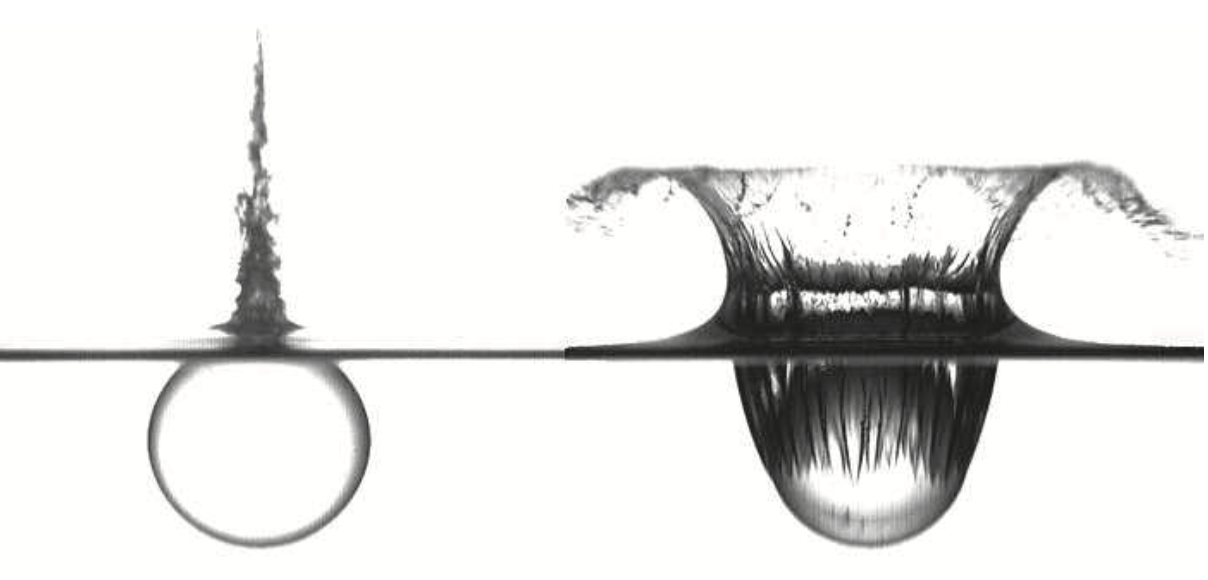
\includegraphics[width=11cm]{duez.png}
\caption{Left: a hydrophilic sphere impacts water without creating any significant disturbance. Right: a similar sphere with a nanometre-thick hydrophobic coating creates a significant splash on impact \citep{Duez2007}.}
\label{fig:splash_no_splash}
\end{center}
\end{figure}

We now review the different types of boundary conditions that fluids satisfy at boundaries.
\section{Fluxes at boundaries: impermeability and imbibition}
\begin{figure}[htbp]
\begin{center}
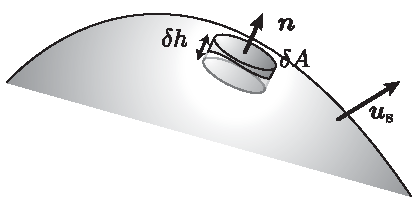
\includegraphics{impermeability.pdf}
\caption{Balance over an elementary volume located across a solid boundary.}
\label{fig:impermeability}
\end{center}
\end{figure}

Let's consider a solid moving in a fluid at velocity $\bu_\text s$ (possibly time dependent) and let's conduct a mass balance on a small cylindrical volume of base $\delA$ and height $\delh$ located across the fluid and the solid (Fig.~\ref{fig:impermeability}). Now let $\delh$ tends to 0 so that the mass element shrinks down to zero.  From now on, the mass variation of the element should necessarily be zero, and this implies that the mass flux from the fluid has to be balanced by the mass flux from the solid side:
\begin{equation}
-\lp\bj_\text{fluid}\cdot \bn_\text{fluid}\rp \delA -  \lp\bj_\text{solid}\cdot \bn_\text{solid}\rp \delA = 0.
\end{equation}
Let's write arbitrarily $\bn = \bn_\text{fluid} = - \bn_\text{solid}$ so that:
\begin{equation}
-\bj_\text{fluid}\cdot \bn +  \bj_\text{solid}\cdot \bn = 0.
\end{equation}
In absence of fluid mixing phenomena, the fluid velocity $\bu$ already takes into account diffusive effects (it is the chemical species velocity) and the mass flux reduces to the convective flux. Beware that as we are in the solid reference frame, the relative velocity of the fluid is $\bu - \bu_\text s$, so that the mass flux on the fluid side is:
\begin{equation}
\bj_\text{fluid} = \rho \lp\bu-\bu_\text s\rp.
\end{equation}
\prg{The impermeable wall.\index{boundary conditions!impermeability}} A very common case is that of an \textbf{impermeable} solid in which the fluid cannot penetrate; the fluid mass flux within the solid is therefore zero and $\bj_\text{solid} = \boldsymbol 0$. Mass conservation expressed at an impermeable boundary therefore reduces to:
\begin{equation}
\bu\cdot\bn = \bu_\text s \cdot\bn
\label{eq:impermeability}
\end{equation}
This is the \textbf{impermeability condition} for an object (or a wall). As the name implies, it simply expresses the fact that the fluid cannot penetrate into the solid. This condition takes the form of a \textbf{continuity of normal velocities}.

Note: in the quite particular (but still very common!) case of a fixed solid object, this condition reduces to $\bu\cdot\bn =0$.
\prg{Permeable wall.}\index{boundary conditions!imbibition} The previous discussion naturally extends to the case of permeable walls. Those may correspond to biological tissues permeable to given solutes, to materials swollen by solvents, to terrains soaked by rain or to lifting sails or wings made porous in order to control the boundary layer (such as Cousteau and Malavard' turbosail\index{turbosail} seen in the lecture, see also Fig.~\ref{fig:turbosail}).
\begin{figure}[htbp]
\begin{center}
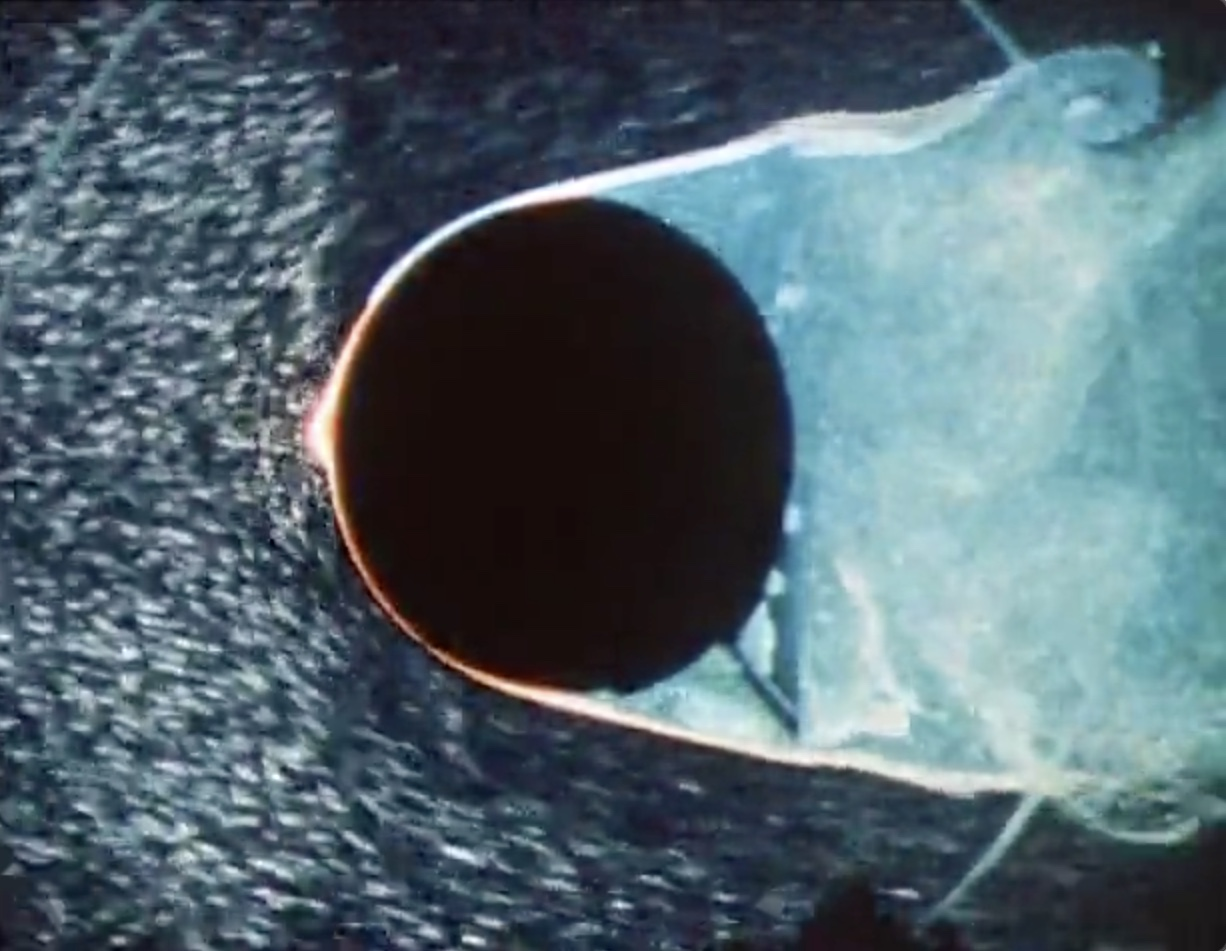
\includegraphics[width=4cm]{cylinder_without_suction.jpg}
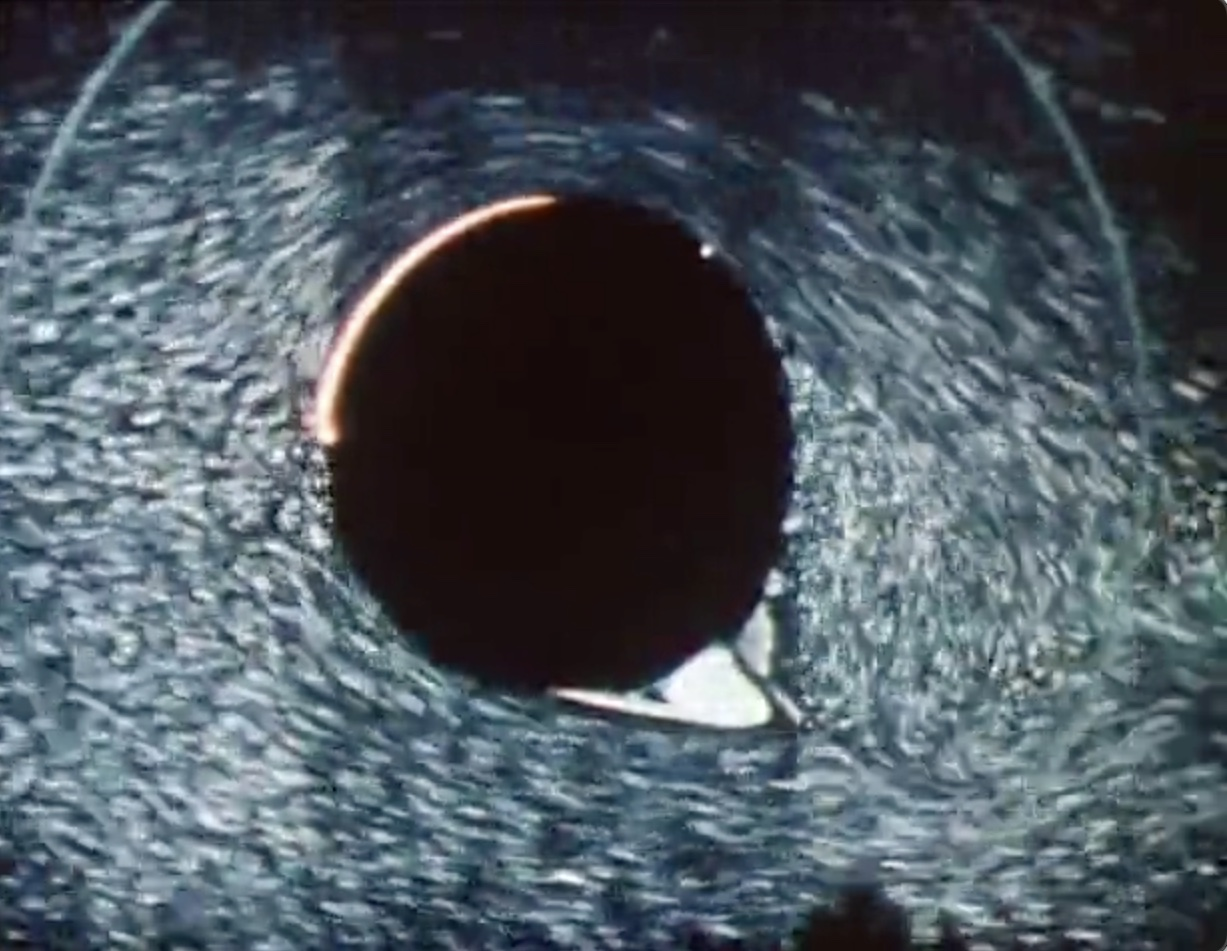
\includegraphics[width=4cm]{cylinder_with_suction.jpg}
\caption{Left: A cylinder placed in a crossflow exhibits a wide wake, associated with an important inertial drag force. Right: with an appropriate suction on the cylinder' surface, the flow reattaches and a significant lift is now obtained. This is the underlying principle of the \textbf{turbosail}. Experiments performed in Malavard's lab at ONERA (excerpt from the movie \href{https://dai.ly/x16epb4}{Écoulements tourbillonnaires d'une maquette de turbovoile - 1984}).}
\label{fig:turbosail}
\end{center}
\end{figure}

Now the mass flux is non-zero and its precise determination requires a knowledge of the flow \textit{inside} the solid. Suppose however that the imbibition velocity $\bu_\text{imbib}$ be constant and known (this corresponds for example to a suction with an imposed flowrate). The mass conservation at the permeable wall will then be written:
\begin{equation}
\rho (\bu-\bu_\text s) \cdot \bn = \rho (\bu_\text{imbib}) \cdot \bn,
\end{equation}
thus 
\begin{equation}
\bu\cdot\bn = \lp\bu_\text s + \bu_\text{imbib}\rp\cdot\bn.
\end{equation}
\prg{Boundary conditions on a concentration field near a wall.\index{boundary conditions!no-flux}}
The boundary conditions to apply on the transport equation of a concentration field~(\ref{eq:conv_diff}) can be obtained following the same principles. Imagine a concentration field transported with a fluid flow $\bu$. Suppose also that an (impermeable) solid is moving in the fluid at velocity $\bu_\text s$. In the solid reference frame the mass flux across any surface $\delA \,\bn$ is:
\begin{equation}
\bj_\text{mass} = \bj_\text{conv} + \bj_\text{diff} = c \lp \bu - \bu_s\rp - D \nabla c.
\end{equation}
The impermeability condition at the wall for the concentration field $c$ is therefore:
\begin{equation}
c (\bu-\bu_\text s) \cdot \bn - D \nabla c \cdot \bn = 0,
\end{equation}
because the mass flux inside the solid is zero.
On using the impermeability condition on the velocity field~(\ref{eq:impermeability}), this relation reduces to:
\begin{equation}
\nabla c \cdot \bn \equiv \pd{c}{n} = 0.
\end{equation}
This Neumann condition is also called a \textbf{no-flux boundary condition.}
\prg{Mass transfer at an interface: evaporation.\index{boundary conditions!evaporation}} One last example of boundary conditions arising from conservation considerations is the continuity of the mass flux across a liquid-gas interface, when the (single-phase) liquid is evaporating.

Let's write a mass balance on a fluid element analogous to the previous one: a small cylindrical element of base $\delA$ and height~$\delh$ located across a moving interface with velocity $\bu_\text i$. We let the height $\delh$ of the element tend to zero, so that the element mass equally tends to zero. The mass balance over this element is:
\begin{equation}
\bj_\text{liquid conv.} \cdot \bn = \lp\bj_\text{gas conv.} + \bj_\text{gas diff.}\rp \cdot \bn
\end{equation}
so that :
\begin{equation}
\underbrace{\rho_\ell \lp\bu_\ell - \bu_\text i\rp \cdot \bn}_\text{interface ablation} = \underbrace{\rho_v \lp\bu_g -\bu_\text i\rp\cdot \bn}_\text{Stefan's flow} \underbrace{- D \nabla \rho_v \cdot n}_\text{diffusive mass flux}.
\label{eq:evaporation_BC}
\end{equation}
From this balance it is apparent that the interface evaporation is driven by two contributions: a convective mass flux and a diffusive one. The convective, so-called Stefan flow from the the expansion of liquid solvent into vapour solvent. 
In the context of a violent evaporation (e.g. boiling, combustion front), this is the dominating contribution and from the balance relation we that in this context:
$$\bu_g \sim \underbrace{\frac{\rho_\ell}{\rho_v}}_{\gg 1} \bu_\ell.$$
However in the other limit where evaporation is very slow, which corresponds to everyday life situations, such as the slow drying of a water drop in plain air, this is the reverse. The diffusive mass flux largely overrides the convective (Stefan) flux, so that it can safely be disregarded\footnote{It can be shown that the ratio between Stefan over diffusive flow is simply the mass fraction of solvent in the gas near the interface \citep{Magdelaine2019}. When a liquid is boiling, the air surrounding the interface is pure solvent vapour, so this mass fraction is of order 1 and Stefan's flow contribution becomes important. Conversely, the saturation vapour pressure of water at ambient temperature is 2.3 kPa -- corresponding to a mass fraction of water vapour in air of 1.5 \%. In this limit, the contribution of Stefan's flow is negligible to describe evaporation.}.
\prg{Application: drop evaporation and D$^2$-law.}\index{drop!evaporation} We can build up on the previous considerations to provide with an estimate of the time it takes for an isolated and still water drop to evaporate in plain air. At first sight, we might be tempted to scale the overall mass loss rate of the drop with its surface $\propto R^2$, and conclude that the radius of the drop decreases linearly with time. However this is not so, because the diffusive transport of water away from the drop sets a bound on how fast the drop evaporates: drop evaporation is an example of a \textbf{diffusion-limited} problem. Drop evaporation in still air was first investigated by \citet{Maxwell1890} who was interested in developing a theory of the wet bulb thermomether -- a curious and ingenious device aimed at measuring air humidity. \citet{Langmuir1918} obtained the very same result years later, without apparent knowledge of Maxwell's former investigations.

Considering a still drop with no motion at constant temperature\footnote{This is arguably a fragile hypothesis, as the latent heat of evaporation is responsible for an overall cooling down of the drop. While D$^2$'s law is found to hold, the prefactor of the law becomes non-trivial when taking all effects into account, see \citet{Cazabat2010} for a discussion.}, we can rewrite the boundary condition~\eqref{eq:evaporation_BC} at the surface of the drop as:
\begin{equation}
\rho_\ell \dd{R}{t} = D \left.\pd{c}{r}\right|_{r=R}.
\label{eq:drop_recoil}
\end{equation}
Here we neglected Stefan's flow contribution, and benefited from the spherical symmetry of the problem to project it along~$\be_r$. The velocity of the interface has been replaced with the rate of variation of $R$, and we have denoted $c$ the water vapour concentration, and $D$ its diffusion coefficient in air. It is apparent from this expression that $R$ is directly driven by the vapour density profile in air, which itself is set by diffusion. 
Introducing air's humidity $\mathcal H$ such that $c = c_\text{sat} \mathcal H$, we may also rewrite this boundary condition as:
\begin{equation}
\dd{R}{t} = D \frac{c_\text{sat}}{\rho_\ell} \left.\pd{\mathcal H}{r}\right|_{r=R}.
\label{eq:drop_recoil_humidity}
\end{equation}
Humidity is a dimensionless quantity equal to 1 at the drop' surface, and 0 in dry air (typically this is the value at infinity).
To make progress, it is therefore necessary to look at the diffusion equation for the water vapour:
\begin{equation}
\pd{\mathcal H}{t} = D\frac{1}{r}\frac{\partial^2}{\partial r^2}\left(r \mathcal H\right).
\label{eq:water_vapour_diffusion}
\end{equation}
A quick order of magnitude estimate for the diffusion profile build-up reads:
$$
\tau_\text{diff} \sim R^2/D,
$$
as pure dimensional analysis could have revealed immediately. This characteristic timescale may conveniently be compared to the drop evaporation timescale, estimated with an order of magnitude analysis from~\eqref{eq:drop_recoil_humidity}:
\begin{equation}
\frac{R}{\tau_\text{evap}} \sim D \frac{c_\text{sat}}{\rho_\ell} \frac{\Delta \mathcal H}{R}.
\label{eq:evaporation_quick_estimate}
\end{equation}
Here $\Delta \mathcal H$ is typically of order 1. Rearranging we have:
$$
\frac{\tau_\text{diff}}{\tau_\text{evap}} \sim\frac{c_\text{sat}}{\rho_\ell}.
$$
For water in air at ambient temperature, $c_\text{sat} = 1.7 \times 10^{-2}$ kg/m$^3$, whereas $\rho_\ell = 1000~$kg/m$^3$. This indicates that evaporation is very slow with regards to diffusion build-up: the water vapour profile adjusts almost instantaneously as the drop shrinks. This justifies the search of a steady-state water vapour profile for \eqref{eq:water_vapour_diffusion}:
\begin{equation}
\mathcal H(r) = \frac{R}{r} \Delta \mathcal H + \mathcal H_\infty,
\end{equation}
with $\Delta \mathcal H = 1 - \mathcal H_\infty$.
This humidity field allows to rewrite~\eqref{eq:drop_recoil_humidity} as:
\begin{equation}
\dd{R}{t} = - D \frac{c_\text{sat}}{\rho_\ell} \frac{\Delta \mathcal H}{R},
\end{equation}
from which we obtain the radius evolution:
\begin{equation}
R(t) = \left(R_0^2 - 2 D \frac{c_\text{sat}}{\rho_\ell}\Delta \mathcal H t\right)^{1/2},
\end{equation}
a result known as \textit{D$^2$-law of evaporation} (so called because the diameter squared of the drop decreases linearly with time). The timescale of an isolated, evaporating droplet follows:
\begin{equation}
\tau_\text{evap} = \frac{1}{2}\frac{R_0^2}{D} \frac{\rho_\ell}{c_\text{sat}} \frac{1}{\Delta \mathcal H},
\end{equation}
a result consistent with our quick order of analysis estimate~ \eqref{eq:evaporation_quick_estimate}.
%fixme: add d2 law for evaporating droplets (e.g. Cazabat et al.) -> tutorial?
\section{Phenomenological conditions: adherence and continuity}
In addition to the previous boundary conditions arising from conservation principles, fluids are also subject to other boundary conditions as well. The latter have been established and confirmed on experimental grounds, so there is a consensus about their relevance but not an exact demonstration. These phenomenological conditions are \textbf{field continuity conditions} at interfaces and apply on velocity, temperature etc.

\paragraph{$\rhd$ A short history of adherence.\index{boundary conditions!adherence}} The adherence condition $\bu = \bu_\mathrm{s}$ has an astonishing history full of twists and turns, which is accounted for in details in \citet{Goldstein1950}. At the \textsc{xviii}$^\text{th}$ century, the theoretical description of potential flows (corresponding to the idealisation of perfect flow of fluid) was already well established, but the comparisons with experimental data were mediocre. Daniel Bernoulli was well aware of this fact and attributed the discrepancies between (ideal) predicted flows and those observed to some ``adherence condition'' that would prevail at the wall. Coulomb then demonstrated experimentally that a disk oscillating in a liquid was not particularly affected by a change in surface properties (smooth, rough or covered with grease). Therefore it appeared to Coulomb that the fluid velocity matched the disk velocity in its vicinity. In this vision the fluid has the same properties in every point of space; the flow just fulfils an additional condition at the wall.

But during the \textsc{xix}$^\text{th}$ century alternate theories appeared. Girard proposed that the liquid layer adjacent to a wall had differing physical properties, leading it to adhere the solid. The next fluid layer (composed of ``regular fluid'') could then freely slip onto the first affixed layer. Navier also got interested into this problem and suggested a boundary condition involving a slip directly proportional to the shear stress $\beta u = \mu \pd{u}{n}$. Here the ratio $\mu/\beta$ has the dimension of a length: it is the \textit{slip length}. From there a period of relative confusion ensued where famous theoreticians of the time (Poisson, Stokes) alternately adopted one or the other of the boundary conditions.

With time however, delicate experiments conducted by Couette or Maxwell advocated definitely for the adherence condition. Maxwell suggested on molecular dynamics considerations that if Navier's condition was effectively valid, the length over which slip occurred was so small -- of the order of a few mean free paths -- that considering it to be zero was a really reasonable hypothesis. This amounted to consider adherence at the wall: $\bu = \bu_\text s$ \citep{Maxwell1879}. This is in particular verified in the usual conditions of laboratory experiments, but not necessarily for rarefied gas flows (e.g. atmospheric reentry, hypersonic flight) or flows involving fluids with long polymer chains (microfluidic flows), as experiments confirm \citep{Henot2018}.
%fixme: add ref on polymer slip

During the \textsc{xx}$^\text{th}$ century, the almost perfect agreement between experimental observations and theoretical predictions using adherence condition for a number of flows (Poiseuille flow, Couette flow, Stokes' sphere settlement in a viscous fluid, the instability threshold for the Taylor-Couette experiment etc) definitely settled the validity of this condition.

Moreover, the scaling laws for the drag on an object deduced from dimensional considerations based on the characteristic scales $\rho, U, D$ and $\mu$ capture the evolution of aerodynamic forces over a wide range of scales. If another lengthscale (associated with slip) was relevant in the description of conventional flows, it would result in an alteration of the scaling laws (not observed).

We can understand adherence condition (continuity of $\bu$ across an interface) but also the condition on temperature continuity as resulting from equilibrium at the molecular level. The extremely rapid transfers between neighbouring molecules induce a quasi-instantaneous equilibrium of mean momentum (velocity) and mean thermal agitation velocity (temperature) \citep{Batchelor1967}. At an interface between a medium \textsc{i} and a medium \textsc{ii} (solid-fluid, or fluid-fluid), we will therefore get:
\begin{equation}
\bu_\text{\textsc{i}} = \bu_\text{\textsc{ii}} \quad \text{and} \quad T_\text{\textsc{i}} = T_\text{\textsc{ii}}.
\end{equation}

\section{Where is the interface?}
A wide range of flows are associated with interfaces: avalanches, rivers, oceans, emulsion droplets, rain or ink drops etc. As we shall see, an interface between a liquid and another fluid is not just an immaterial boundary geometrically delimiting portions of space occupied by fluids. An interface is an \textbf{active region} where surface tension forces act, in some way analogous to those exerted by a taut membrane.

But before precising the nature of these forces acting on the interface, we first need to be able to know where the interface is! Indeed, an interface is constantly moving by definition and we have to start tracking the interface through time and space. This is the purpose of the \textit{kinematic boundary condition} which will allow us to follow the interface in its motion.
\subsection{Kinematic boundary condition.\index{boundary conditions!kinematic}} In order to describe the motion of any given interface, as a free surface for example, let's introduce an arbitrary function $\mathcal S(\bx,t)$ that vanishes on the interface at all times: for each point $\bx_\text{interf}$ of the interface,~$\mathcal S(\bx_\text{interf},t)~=~0$. Between two successive instants, an interface point is displaced with a distance $\delbx = \bu_\text i \delt$ and:
\begin{equation}
\mathcal S(\bx_\text{interf} + \bu_\text i \delt, t + \delt) \approx \underbrace{\vphantom{\lp\pd{\mathcal S}{t}\rp}\mathcal S(\bx_\text{interf},t)}_0 + \delt\underbrace{\lp\pd{\mathcal S}{t} + \lp\bu_\text  i \cdot \nabla\rp\mathcal S\rp}_{\dd{_\text i\mathcal S}{t}} = 0.
\end{equation}
To get the interface velocity $\bu_\text i$\footnote{We note that in the expression of $\mathcal S$, only the normal component $\bu_\text i \cdot \bn$ of $\bu_\text i$ at the interface is involved.} we just need to express the mass flux boundary condition at the interface. If there is no mass transfer at the interface (such as e.g. evaporation), the latter reads:
\begin{equation}
\rho \lp \bu - \bu_\text i\rp \cdot \bn = 0 \quad \text{thus} \quad \bu \cdot \bn = \bu_\text i \cdot \bn,
\end{equation}
so that the kinematic boundary condition describing the motion of a free surface simply reads:
\begin{equation}
\dd{\mathcal S}{t} = 0
\end{equation}
\prg{Example: description of a free surface.} Consider a free surface such as the ocean's, characterised\footnote{We here suppose that the interface is single valued (no wave breaking!).} with $z = \zeta(x,y,t)$. The surface is described at each instant by the vanishing of the function\footnote{We could imagine other functions as well, e.g. $\mathcal S(\bx,t) = \tanh\lp z - \zeta\lp x,y,t\rp\rp$ \ldots} :
\begin{equation}
\mathcal S(\bx,t) = z - \zeta(x,y,t).
\label{eq:bumped_free_surface}
\end{equation}
The kinematic boundary condition describing the position of the free surface is therefore:
\begin{equation}
\dd{\mathcal S}{t} = 0 \quad \text{hence}\quad \pd{\zeta}{t} = u_z - u_x \pd{\zeta}{x} - u_y \pd{\zeta}{y}
\end{equation}
\subsection{Surface geometry I. Normals.\index{normal vector}} In a number of problems involving free surfaces, deformable and/or complex boundaries, the expression for the normal vector has to be provided. A systematic procedure to obtain the expression for this vector stems in remarking that the free surface coincides with a $\mathcal S$-isosurface. As a result the normal vector is necessarily parallel with the \textbf{gradient} of $\mathcal S$ :
\begin{equation}
\bn = \frac{\nabla \matS}{\|\nabla \matS\|}
\end{equation}
\prg{Example: free surface normal.} Let's consider the previous example again. We have:
$$
\nabla \matS = \lp
\arraycolsep=1.4pt\def\arraystretch{1.5}
\begin{array}{c}
-\pd{\zeta}{x}\\
-\pd{\zeta}{y}\\
1
\end{array}
\rp,
$$
so
\begin{equation}
\bn = \frac{1}{\sqrt{1+\pd{\zeta}{x}^2+\pd{\zeta}{y}^2}}\lp
\arraycolsep=1.4pt\def\arraystretch{1.5}
\begin{array}{c}
-\pd{\zeta}{x}\\
-\pd{\zeta}{y}\\
1
\end{array}
\rp.
\label{eq:wave_normal}
\end{equation}
We note the the direction of this normal is quite arbitrary and chosen by convention (usually, the convention is that of exterior-pointing normal. However this only makes sense if the very notion of exterior makes sense!).

\section{Capillarity\index{surface tension}}
\begin{figure}[htbp]
\begin{center}
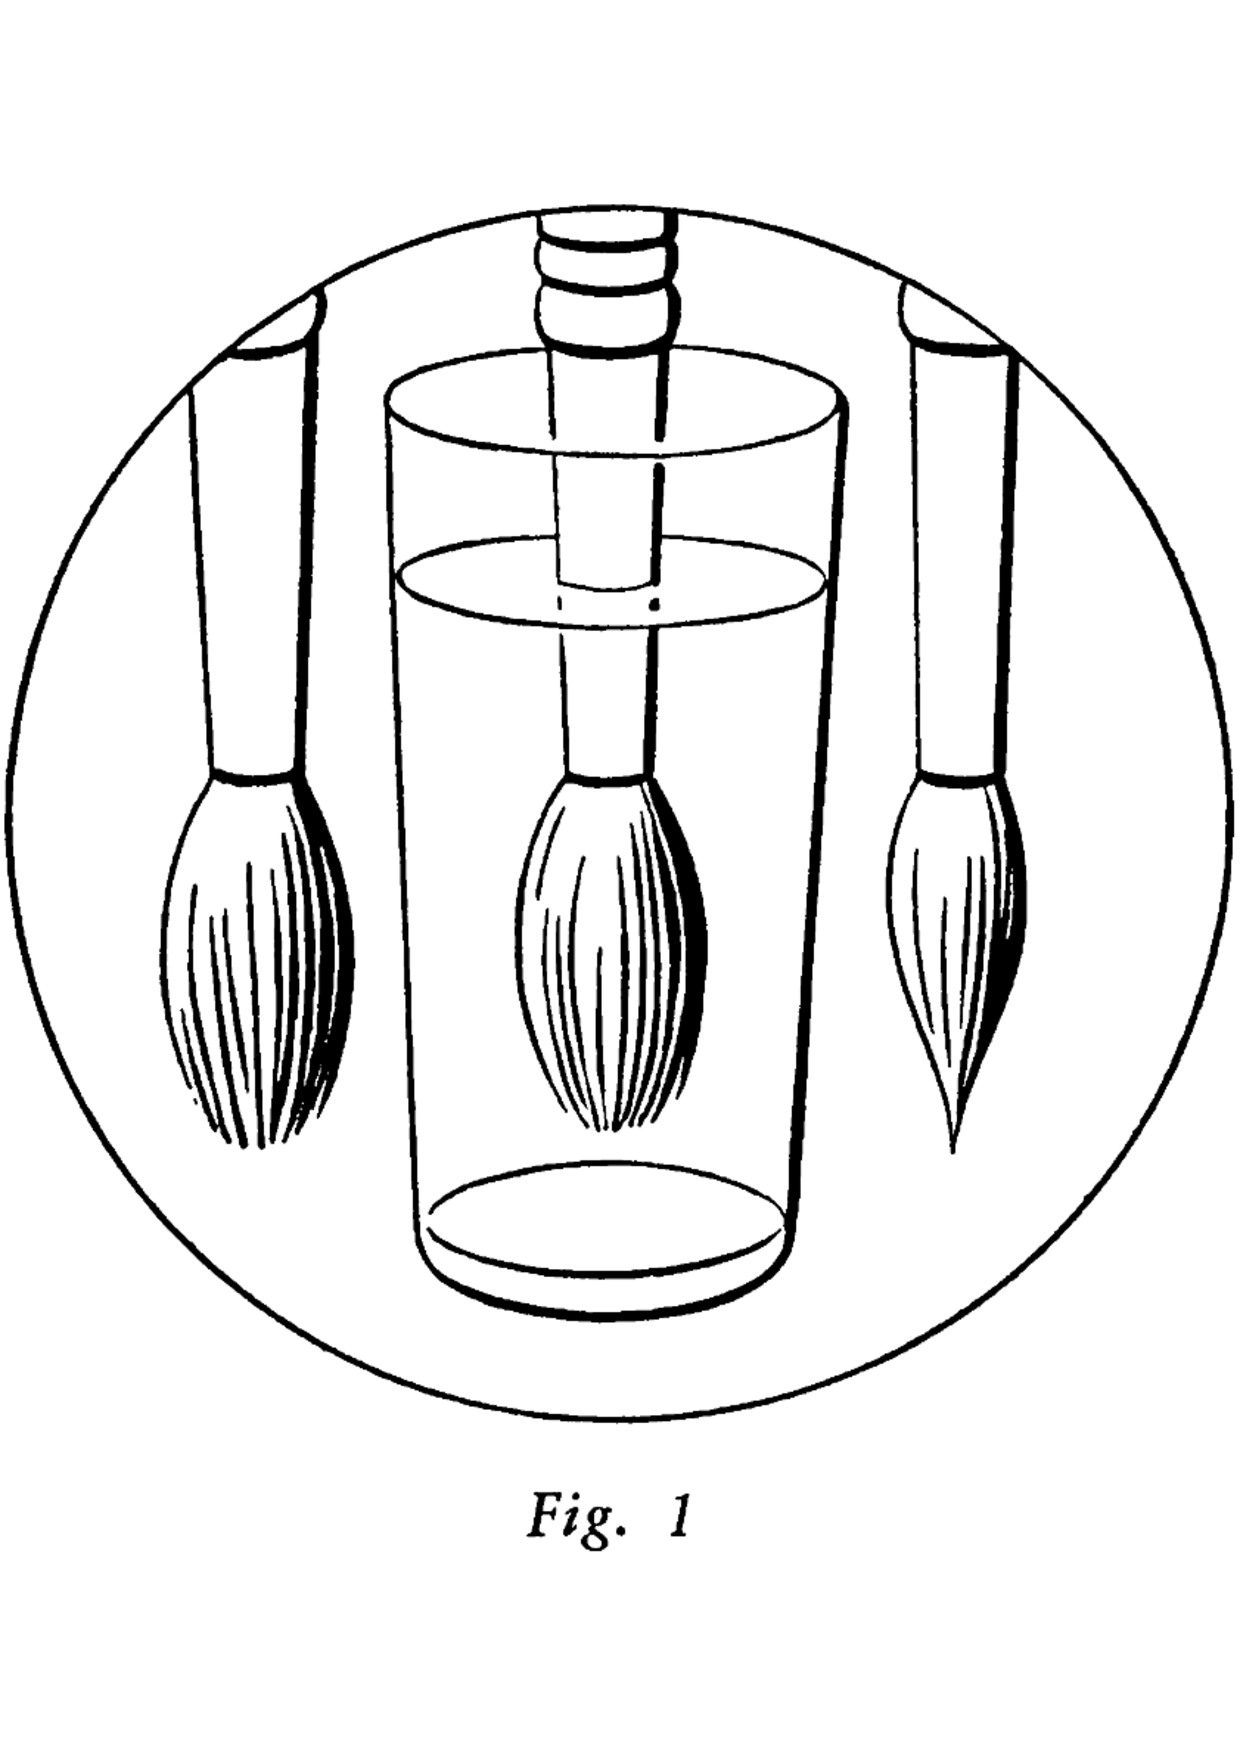
\includegraphics[width=4cm]{boys_brush.pdf}\\
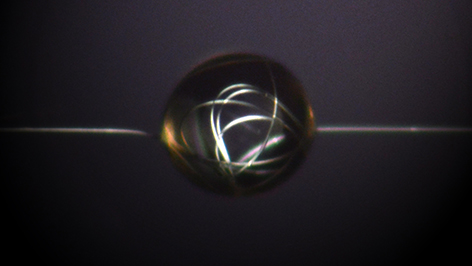
\includegraphics[height=4cm]{capillary_spool_downsampled.jpg} \quad
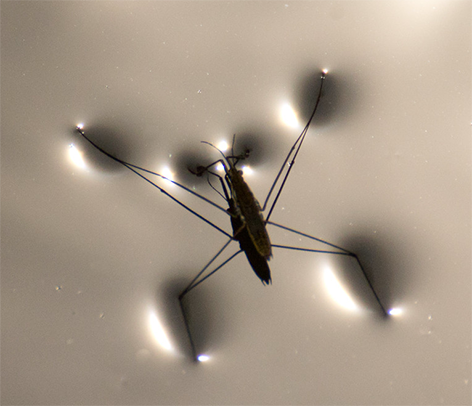
\includegraphics[height=4cm]{gerris_on_water_downsampled.png}
\end{center}
\caption{Top: when pulled out of water, a wet brush has its bristles stuck altogether, but those are neatly separated is the brush is dry or fully immersed \citep{Boys1890}. Bottom left: a drop deposited on a sufficiently thin fibre such as the spider capture silk induces coiling and spooling within the droplet \citep{Elettro2016}. Bottom right: the Gerris, an aquatic insect, can literally walk on water although it is denser (\href{https://www.flickr.com/photos/ryoichi360/5847533955/in/photolist-9UJ97X-EU3vy-V3eJzF-8wimyD-fafpgs-HKfkdJ-22TUHgL-SWUure-dcK4vX-2baXF3n-DhVeuP-rMc5KH-253wqN-2fQ2VWT-8p2CBK-8d9rrm-VmimZt-PcW89C-283Sj59-Hvg77b-N9Ytvw-SN5EhR-cQ7gBj-s4aR9q-eDcCJz-HrEa1e-6hizYZ-Wq8cWg-FYhg7k-8874aQ-iJqVV-56yPYc-X5ffoi-pkU5Zt-p9ztvz-ZSJkzJ-ofYXjT-a9n3xT-2ekD2e9-5sAmFu-ccGJis-24KoY9K-QZW2Li-4f9Fjc-fyuZPT-Hr29p5-kLdZ8n-Tu8m9W-nQg4Lr-s85mcc}{photograph by Ryoichi on Flickr}). These examples are manifestations of surface tension exerted at liquid-gas interfaces.}
\label{fig:surface_tension}
\end{figure}
Having described kinematically interfaces (i.e. how to locate them) along with the boundary conditions resulting from mass conservation and molecular equilibria (adherence condition), we shall now get interested into the dynamical aspects of interfaces and more particularly to the phenomenon of \textit{capillarity} \citep{de-Gennes2015}.

An interface between two immiscible fluids, as that between air and water is, is a material surface separating the two media. But actually such an interface is in reality way more that a simple geometric place delimiting two portions of space. An interface \textbf{bears forces} whose manifestation is visible in daily-life examples, such as the clogging of wet hairs, the spooling of spider thread within glue droplets or the sustentation of small aquatic animals such as the Gerris (Fig.~\ref{fig:surface_tension}).

\subsection{Cohesion}
The microscopic origin of surface tension is rooted in \textbf{cohesion} effects in liquids. Indeed, atoms or molecules that constitute matter interact with each other with forces of changing nature. Repulsive at very short distance, the forces become attractive at longer range. In the context of a gas, the intermolecular distances are far too large for these interactions to have any notable effect. But this is not true for dense phases such as liquids where molecules attract each other. This matter cohesion phenomenon is responsible for the rounded shape of droplets, the curvature of menisci or that of soap films. The history of the link between attractive forces and surface tension is already present in the writings of Newton, but this link was not really elucidated until Laplace in 1805 \citep{Laplace1805}. With the unique hypothesis of attractive forces between two matter particles decaying with distance, Laplace succeeded in finding with differential calculus all equilibria shapes of interfaces. He also explained the capillary rise in tubes, a phenomenon resisting understanding so far \citep{Rowlinson2005}. He further evidenced a pressure jump phenomenon (normal stress) proportional to curvature, as we shall now see.
\subsection{Surface tension}
In parallel to Laplace's works on cohesion and capillarity, Thomas Young also managed to find in 1805 a result on the pressure jump across interfaces identical to Laplace's finding. But he followed an entirely different route \citep{Young1805}. On the basis of experimental observations of free surface deformations similar to those of elastic membrane, Young postulated the existence of a tension force localised at the liquid surface, and analogue to membrane tension -- such as the one developing in a stretched balloon. Following this reasoning, a small, flat and rectangular surface element $\delta S = \delta \ell_1 \delta \ell_2$ such as the one illustrated figure~\ref{fig:flat_surface} would be subject to a total force:
$$
\lp \gamma \delta \ell_2 - \gamma \delta \ell_2 \rp \be_1 + \lp \gamma \delta \ell_1 - \gamma \delta \ell_1 \rp \be_2 = \boldsymbol 0.
$$
As a matter of fact, each force contribution is balanced by another because the surface is flat. But we feel here that this result may change as soon as the surface will be curved. Before proceeding in the estimation of the surface tension force for a general surface, we have to characterise the curvature of a surface.
\begin{figure}[htbp]
\begin{center}
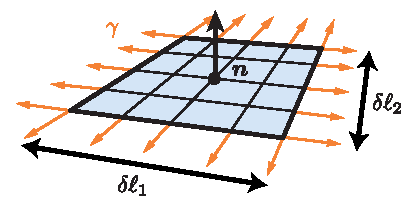
\includegraphics{flat_surface_poly.pdf} \end{center}
\caption{A flat interface portion is subject to a tension force at its periphery.}
\label{fig:flat_surface}
\end{figure}

\subsection{Surface geometry II. Curvature.\index{curvature}}
\begin{figure}[htbp]
\begin{center}
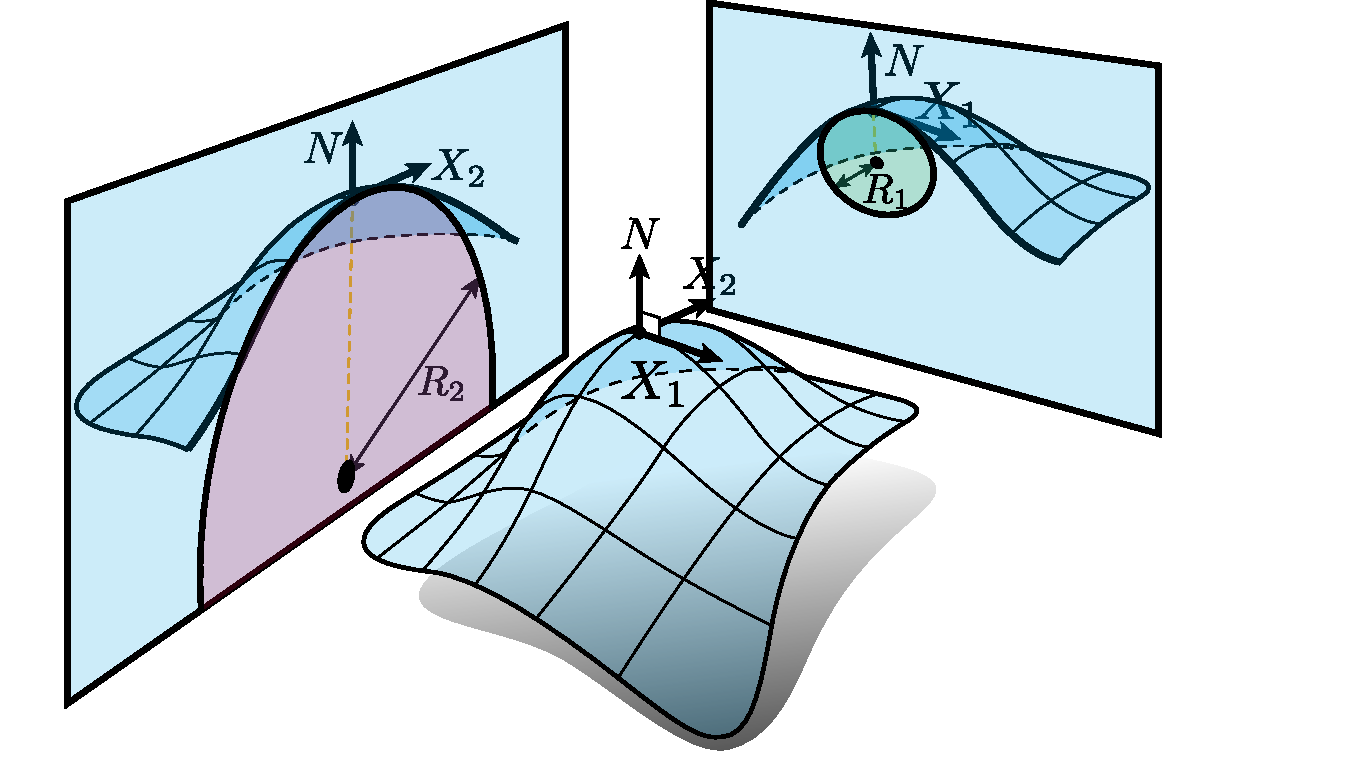
\includegraphics[width=10cm]{principal_curvature.pdf} 
\end{center}
\caption{A curved surface portion intersected with a plane displays different radii of curvature depending on the plane orientation.}
\label{fig:principal_curvature}
\end{figure}
Let's consider the portion of curved interface represented figure~\ref{fig:principal_curvature}. The curvature of the surface on a given point is a geometric quantity that can be built as follows. Start by identifying the normal $\bn$ to the surface at the chosen point. Consider now two perpendicular planes that each contain $\bn$. Each plane will intersect the surface following a curve which may be approximated by a circle in the vicinity of the chosen point. Of course the circle radius will differ in each plane in the general case: we will note it for example $R_1$ in the plane $\lp\be_1,\bn\rp$ and $R_2$ in the plane $\lp\be_2,\bn\rp$. The \textbf{mean} (or arithmetic) \textbf{curvature} $\kappa$ of the surface at the considered point is defined as the sum of the two circle curvatures :
\begin{equation}
\kappa \equiv \frac{1}{R_1} + \frac{1}{R_2}.
\end{equation}
This definition calls for two remarks. The first one regards the unicity of $\kappa$'s definition. Indeed we might envisage another set of two orthogonal planes, each of them also containing $\bn$ (obtained via a simple rotation around $\bn$). We would then get two other values for $R_1$ and $R_2$. Remarkably, it can be shown in surface geometry that if $R_1$ and $R_2$ are not defined in an univocal way, the sum $\frac{1}{R_1} + \frac{1}{R_2}$ is independent of the planes choice! The curvature $\kappa$ is a surface \textbf{invariant} (except in ill-defined cases, such as surfaces with cusps or corners -- in which case the curvature diverges). The second remark is about the curvature sign. Curvature radii are signed quantities, considered positive by convention if the curvature centre is inside the surface, and negative otherwise (to differentiate what is inside from what is outside, we still use the exterior normal convention). It is therefore possible to have a surface of negative curvature.

\prg{Curvature of a sphere.}
To illustrate this notion, let's consider a simple sphere of radius $R$. 
\begin{figure}[htbp]
\begin{center}
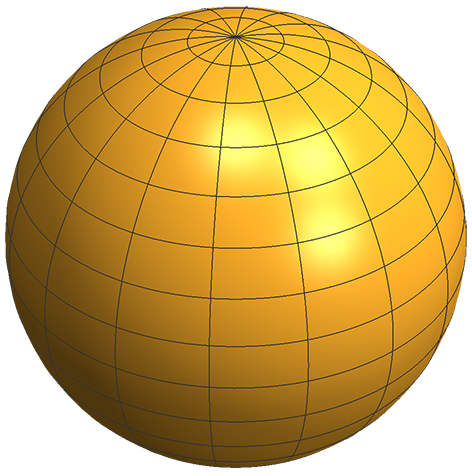
\includegraphics[width=4cm]{sphere_undeformed.png} 
\end{center}
\caption{A sphere.}
\label{fig:sphere}
\end{figure}
At a given point of the surface, the normal vector is given by $\be_r$ and the two perpendicular planes intersecting the sphere will be two (exact) circles each of radius $R$. As a consequence we will have:
\begin{equation}
\kappa_\text{sphere} = \frac{2}{R}.
\end{equation}

\prg{Extension to general surfaces.}
The previous approach, although visual and making direct contact with the meaning of curvature, suffers from some shortcomings. Indeed, beyond elementary shapes (cylinder, cone, axisymmetric surfaces etc) it appears difficult to identify the relevant curvature radii for more general surfaces, such as the wavefield described by equation~\eqref{eq:bumped_free_surface}.

Fortunately there exists an alternate definition for the curvature that comes from surface differential geometry. This alternate definition allows for an easy computation of curvature in every situations:
\begin{equation}
\kappa \equiv \nabla_s \cdot \bn.
\end{equation}
Here the operator $\nabla_s$ represents the surface divergence. In practice we will calculate the (full) divergence of the vector field~$\bn$ defined in every point of space, and then simply consider the restriction of this field at the interface. Now an example to shed some light over this definition.
\prg{Curvature of a sphere (again).} Let's consider again the sphere example. In order to determine $\bn$, we introduce the ``colour function'' $\matS(r) = r - R$. Its normalised gradient gives $\bn = \be_r$ in every point of space -- and in particular at the sphere' surface. The divergence of $\be_r$ reads \textit{in every point of space}:
\begin{equation}
\nabla \cdot \be_r = \frac{1}{r^2} \pd{}{r} \lp r^2 \times 1 \rp = \frac{2}{r}
\end{equation}
The restriction of this field \textit{to the sphere' surface} gives the curvature:
\begin{equation}
\kappa_\text{sphere} = \left.\nabla \cdot \be_r\right|_{r=R} = \left.\frac{2}{r}\right|_{r=R} = \frac{2}{R}.
\end{equation}
\prg{Curvature of a wavefield.} Let's go back to the wavefield equation~\eqref{eq:bumped_free_surface}. The divergence of the normal vector field~\eqref{eq:wave_normal} in each point of space is:
\begin{equation}
\kappa= -\frac{\Delta_\parallel \zeta}{\sqrt{1+\zeta_x^2+\zeta_y^2}} + \frac{\zeta_x\lp\zeta_x \zeta_{xx} + \zeta_y \zeta_{yx}\rp + \zeta_y\lp\zeta_x \zeta_{xy} + \zeta_y \zeta_{yy}\rp}{\lp 1+\zeta_x^2+\zeta_y^2\rp^{3/2}},
\end{equation}
where $\Delta_\parallel \equiv \frac{\partial^2}{\partial x^2} + \frac{\partial^2}{\partial y^2}$ represents the horizontal Laplace operator. We denote in the previous expression differentiation with indices, so that $ \zeta_{yy} = \frac{\partial^2\zeta}{\partial y^2}$. We see that it would have been difficult to establish this relation with circles tangenting the surface! We finally note that in the limit of slender slope, where $\zeta_x,\zeta_y$ are \textit{a priori} much smaller than 1, the expression simplifies significantly to become
\begin{equation}
\kappa \simeq - \Delta_\parallel \zeta \quad \text{in the limit of slender slopes}.
\end{equation}
Yet another manifestation of Laplace operator!
\section{Young-Laplace's pressure jump}
\begin{figure}[htbp]
\begin{center}
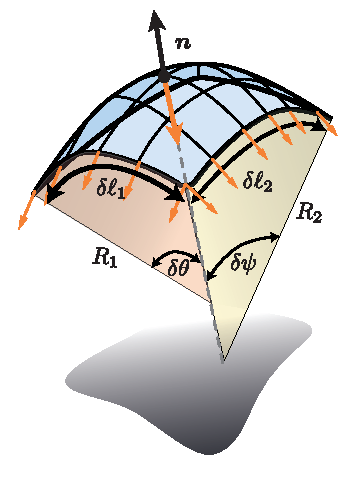
\includegraphics[valign=m,width=6cm]{curved_surface_force.pdf} 
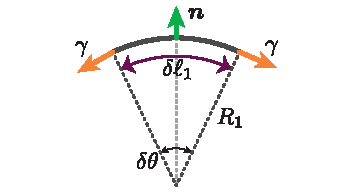
\includegraphics[valign=m,width=8cm]{curved_surface_cut.pdf} 
\end{center}
\caption{Left: a portion of curved interface is subjected to an effective force that depends both on surface tension and on geometry $-\gamma \kappa \, \bn \, \delta S$. Right: sketch of the forces acting on a surface slice showing that contributions along the normal add up.}
\label{fig:curved_surface}
\end{figure}
Having clarified the notion of surface curvature, we can go back to the estimation of the effective surface tension force exerted on a \textit{curved} interface portion. To do so we consider the elementary surface portion described in figure~\ref{fig:curved_surface}. This elementary surface is subtended by two elementary arcs of curvilinear lengths $\delta \ell_1$ and $\delta \ell_2$. To first order the surface is then given by $$\delta S = \delta \ell_1 \delta \ell_2.$$ These two elementary arcs are linked to the two curvature radii $R_1$ and $R_2$ by the infinitesimal angles $\delta \theta$ and $\delta \psi$ represented on figure~\ref{fig:curved_surface} :
\begin{subequations}
\label{eq:curvature_radius}
\begin{empheq}[left=\empheqlbrace]{alignat=2}
\delta \ell_1 \,&=&\, R_1 \delta \theta\\
\delta \ell_2 \,&=&\, R_2 \delta \psi
\end{empheq}
\end{subequations}
To quantify the action of the forces, start by considering the cut indicated on figure~\ref{fig:curved_surface} (right). The two contributions of intensity $\gamma$ are each inclined by $\delta \theta / 2$ with respect to the tangent at the considered point. As a result, the projection along the tangent  $\bt$ and the normal $\bn$ are:
\begin{empheq}[left=\empheqlbrace]{alignat=2}
\text{projection along $\bt$ :} \qquad & \gamma \cos \lp \delta \theta / 2 \rp -  \gamma \cos \lp \delta \theta / 2 \rp = 0\\
\text{projection along $\bn$ :} \qquad & -\gamma \sin \lp \delta \theta / 2 \rp -  \gamma \sin \lp \delta \theta / 2 \rp \simeq -2 \gamma \delta \theta / 2 = - \gamma \delta \theta
\end{empheq}
This is true for each cut along the path $\delta \ell_2$, so that the contribution of surface tension for these two opposite sides is $ -\gamma \delta \theta \delta \ell_2$ along $\bn$. We can repeat this line of reasoning for the two other sides, and we obtain the total contribution of surface tension on this small curved element:
\begin{equation}
\delta \boldsymbol f_\text{cap} = - \gamma \lp \delta \theta \delta \ell_2 + \delta \psi \delta \ell_1 \rp \bn.
\end{equation}
We can reexpress this relation with the help of the curvature radii~\eqref{eq:curvature_radius}:
\begin{equation}
\delta \boldsymbol f_\text{cap} = - \gamma \lp \frac{1}{R_1}\delta \ell_1 \delta \ell_2 + \frac{1}{R_2}\delta \ell_1 \delta \ell_2 \rp \bn,
\end{equation}
so that finally:\footnote{This result could have been obtained directly by application of the \textbf{surface divergence theorem}\index{divergence!surface} which can be stated as:
\begin{equation}
\oint_{\mathcal C} \phi \bp \,\mathrm d\ell = \iint_\mathcal S \nabla_s \phi \,\mathrm dS - \iint_\mathcal S \phi \bn \kappa\,\mathrm dS,
\label{eq:surfdiv}
\end{equation}
where $\mathcal S$ is a portion of a (curved) surface bounded by the contour $\mathcal C$. In this expression $\nabla_s\equiv\nabla-\bn\lp\bn\cdot\nabla\rp$ is the \textit{surface gradient}, and $\bp$ is a vector tangent to the surface but normal to the contour such that $\bp = \bt \times \bn$. This formula is reminiscent of its 3D version $\oiint f \bn \, \mathrm dS = \iiint \nabla f \, \mathrm dV$ except for an extra term involving the curvature of the surface. Actually this extra term may be seen as rooted in a 2D extension of the Frenet-Serret formulae linking curvature, normal and rate of variation of the tangent, see also~\eqref{eq:2Dfrenet}.

\noindent The surface divergence theorem can be demonstrated simply with Stokes' theorem as follows. Let's start by considering a vector field $\bb$ defined on the surface (and not necessarily tangent to the surface -- $\bb$ can really be any vector field). Integrating $\bb\cdot\bp$ on $\mathcal C$ yields:
\begin{alignat*}{1}
\oint_\mathcal C \bb\cdot\bp\,\mathrm d\ell &= \oint_\mathcal C \bb\cdot(\bt\times\bn)\,\mathrm d\ell = \oint_\mathcal C (\bn\times\bb)\cdot\bt\,\mathrm d\ell\\
&= \iint_\mathcal S \nabla\times\lp\bn\times\bb\rp\cdot\bn\,\mathrm dS\\
&=\iint_\mathcal S\lp\bn\lp\nabla\cdot\bb\rp - \bb\lp\nabla\cdot\bn\rp-\lp\bn\cdot\nabla\rp\bb+\lp\bb\cdot\nabla\rp\bn\rp\cdot\bn\,\mathrm dS
\end{alignat*}
The last term here vanishes: this is best seen by writing it using Einstein convention $b_j n_i n_{i,j}$, and remarking that $n_i n_{i,j} = \tfrac{1}{2} \lp n_i n_i \rp_{,j} = 0$ because $n_i n_i = 1$. Now if we take $\bb = \phi \bc$ with $\bc$ an arbitrary \textit{constant} vector, we get:
\begin{equation}
\bc\cdot\left[\oint_\mathcal C \phi \bp\,\mathrm d\ell\right] = \bc\cdot\left[\iint_\mathcal S \lp\nabla \phi -\phi\bn\lp\nabla\cdot\bn\rp-\bn\lp\bn\cdot\nabla\phi\rp\rp\,\mathrm dS \right].
\end{equation}
Upon remarking that for this equation to hold for any $\bc$, the bracket terms have to coincide, and further noting that $\nabla\cdot\bn\equiv\kappa$, we recover~\eqref{eq:surfdiv}.

\noindent Finally, using this expression we see that the correct general expression for $\delta \boldsymbol f_\text{cap}$ is 
\begin{equation}
\delta \boldsymbol f_\text{cap} = \nabla_s \gamma \, \delta S - \gamma \kappa \, \bn \, \delta S,
\label{eq:capillaryforce_marangoni}
\end{equation}
valid for any space-varying surface tension.

\noindent Note: for completeness we might also define a \textit{surface divergence operator} such that the surface divergence of a vector $\bb$ is written 
\begin{equation}
\nabla_s \cdot\bb = \left[\nabla-\bn\lp\bn\cdot\nabla\rp\right]\cdot\bb=\left[\nabla \times (\bn\times\bb)\right]\cdot\bn+(\bb\cdot\bn)(\nabla\cdot\bn).
\end{equation}
With this last expression it becomes apparent that the surface divergence of $\bn$ is just the restriction of the full divergence of $\bn$ to the surface, i.e. $\nabla_s\cdot\bn=\nabla\cdot\bn$ on the surface.
}
\begin{equation}
\delta \boldsymbol f_\text{cap} = - \gamma \kappa \, \bn \, \delta S.
\end{equation}
In other words a small curved surface element will be accelerated towards its curvature centre with a force of intensity proportional to both surface tension and curvature. The force exerted on an element therefore depends on its geometry!

Let's stop for a moment and discuss the consequences of such a force. From the previous expression we might be tempted to conclude that each element of a water droplet is accelerated towards its centre, and that the droplet should collapse onto itself. To understand how droplets and other interfaces can withstand this force and remain at equilibrium, we have to remember that droplets are made of a liquid (e.g. water) that is hardly compressible. In practice this incompressibility constraint is guaranteed\footnote{Note: even in compressible fluids (ex: bubble) a pressure field is established to counterbalance the effect of capillary force.} with the help of a pressure field that will balance the effect of surface tension. Actually, a pressure field is present in the liquid, even at equilibrium. As seen in chapter~\ref{chap:fluid-motion} the pressure force exerted onto the small considered surface element will be: 
$$
\delta \bff_\text{pressure} = \lp p_\text{int} - p_\text{ext}\rp \bn \,\delta S.
$$
The interface portion equilibrium condition will then be:
\begin{equation}
\delta \bff_\text{cap} + \delta \bff_\text{pressure}  = \boldsymbol 0,
\end{equation}
so that\index{Laplace pressure jump}
\begin{equation}
\Delta p = p_\text{int} - p_\text{ext} = \gamma \kappa.
\label{eq:laplace_jump}
\end{equation}
To ensure equilibrium, a \textbf{pressure jump} will be established across an interface. This surprising result, due to Young and Laplace, implies that a millimetric rain droplet can sustain overpressure of $\gamma \kappa \simeq 7 \times 10^{-2} \times \frac{2}{10^{-3}} = 140 $ Pa with respect to the atmosphere, and a micron-sized fog droplet will endure an overpressure of $\simeq 7 \times 10^{-2} \times \frac{2}{10^{-6}} = 1.4\times 10^{5} $ Pa, thus 1.4 bars more than atmospheric pressure!
\subsection{Surface tension?}
We followed in the previous analysis Young's viewpoint according to which the interface would be taut by a constant surface tension $\gamma$. We also recovered Laplace's result of the pressure jump when traversing a curved interface. Laplace did not suppose a distributed surface tension but only attractive forces between molecules. But as we have seen in the previous part, it is possible to switch mathematically from a tangent force representation to an effective normal force, and the reverse. Our demonstration is in fact the expression of a generalisation of Frénet's formulae to three dimensions:
\begin{equation}
\oint_C \bp\,\mathrm d\ell = -\iint_A \kappa \bn\, \mathrm dS,
\label{eq:2Dfrenet}
\end{equation}
where $\bp$ is a vector tangent to the interface and $C$ a closed curve over the interface \citep{Tryggvason2011}. From this, we may wonder if surface tension exists \textit{really}, or if it is not simply a convenient mathematical trick to describe the attractive interactions between molecules.
\begin{figure}[htbp]
\begin{center}
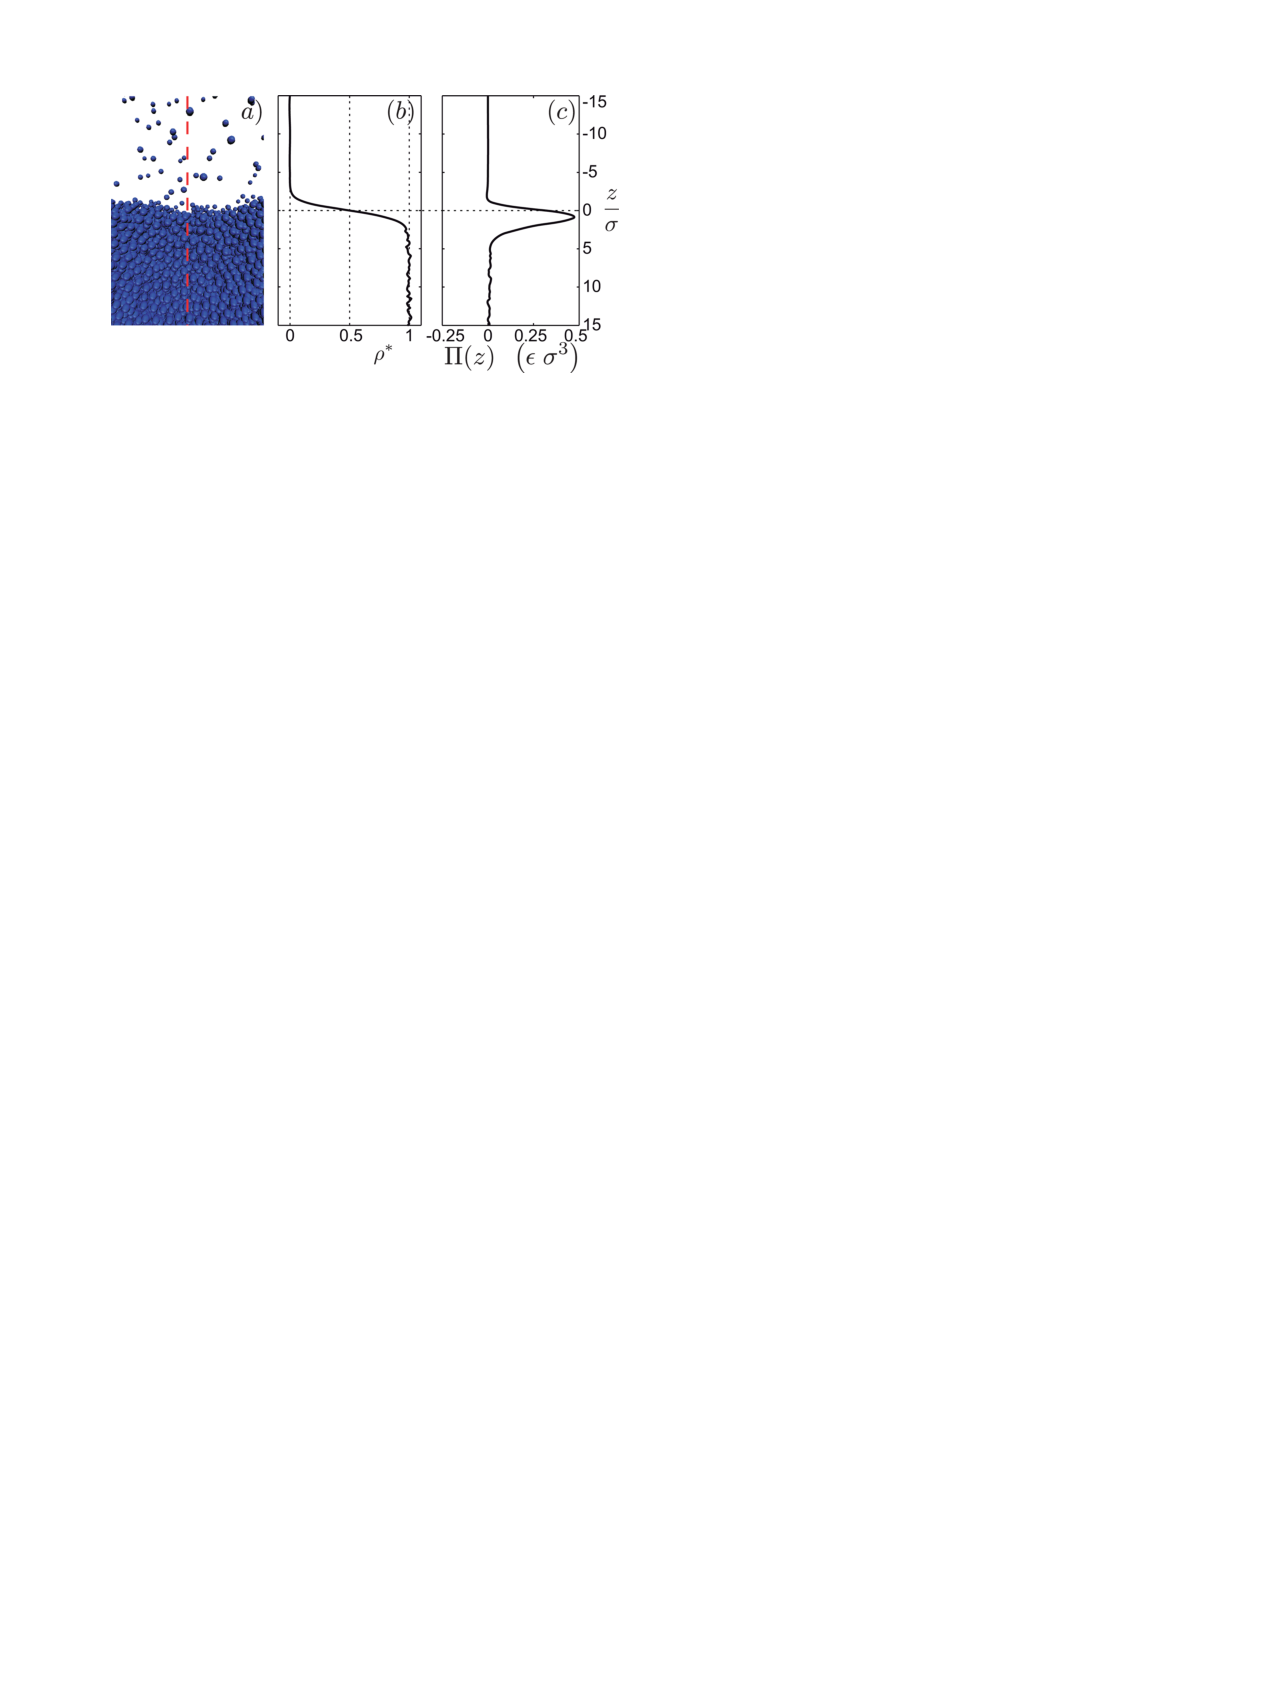
\includegraphics[width=8cm]{marchand_andreotti.pdf} 
\end{center}
\caption{Dynamic molecular simulations show that in the vicinity of an interface, molecules are farther apart than in the liquid bulk. This depletion is associated with an increase of attractive force between molecules at the surface. The macroscopic consequence of this increase is the emergence of surface tension \citep{Marchand2011}.}
\label{fig:marchand}
\end{figure}
It is now possible to use dynamic molecular simulations to answer this question. As shown in figure~\ref{fig:marchand}, there exists a force parallel to the interface that stems from a depletion in near surface molecules: surface tension has therefore a physical reality! \citep{Berry1971,Marchand2011}.
 
%Mais contrairement à une membrane élastique, la \textbf{tension de surface} $\gamma$ d'une interface est constante, quel que soit l'étirement imposé. La valeur de cette tension de surface est très faible -- de l'ordre de quelques dizaines de milliNewtons par mètre tout au plus, mais elle est suffisante pour sculpter des interfaces liquides et conférer, par exemple, une forme sphérique à de petites gouttes d'eau. 

\subsection{Stress (dis-)continuity}
With the notion of \textit{stress}, the previous result may easily be extended to the case of moving interfaces. To do so let's consider an elementary volume in the shape of a camembert box leaning on each side of the interface, see figure~\ref{fig:impermeability}. Now we let the volume thickness tend to 0, so that both the mass and the momentum of the element tend to zero as well. As a result the sum of the forces acting on this volume must be zero as well. We have already seen with~\eqref{eq:capillaryforce_marangoni} that the net sum of interfacial stresses is $\nabla \gamma \, \delta S -\gamma \kappa \, \bn \, \delta S$. The stress exerted by the exterior medium is $\mathsfbfit{\sigma}_\text{ext} \bn_\text{ext} \delta S$, and similarly for the stress exerted by the interior medium $\mathsfbfit{\sigma}_\text{int} \bn_\text{int} \delta S$, with $\bn_\text{ext} = - \bn_\text{int} = \bn$. The condition for interface equilibrium will thus be:
\begin{equation}
\lp\mathsfbfit{\sigma}_\text{ext} - \mathsfbfit{\sigma}_\text{int}\rp \bn = - \nabla_s \gamma + \gamma \kappa \bn.
\end{equation}
This is a really general relation that expresses a \textbf{stress jump} at the interface. Note that in  the particular static case where $\sigij = -p \delij$ with constant surface tension, this relation becomes:
\begin{equation}
\Delta p = p_\text{int} - p_\text{ext} = \gamma \kappa,
\end{equation}
which is naturally the Laplace pressure jump seen in~\eqref{eq:laplace_jump}.

\section{Equilibrium shape for a meniscus\index{meniscus}}
\begin{figure}[htbp]
\begin{center}
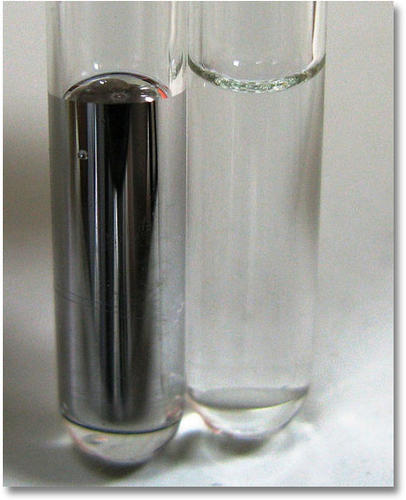
\includegraphics[height=4.5cm]{wss-property-meniscus-water-mercury_0.jpg}
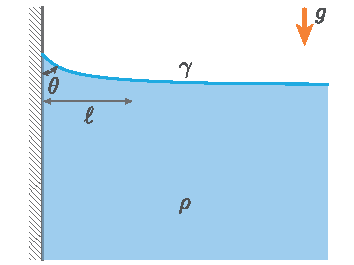
\includegraphics{meniscus.pdf} 
\end{center}
\caption{Left: mercury or water contained in test tubes exhibit sharply different menisci (\href{https://www.usgs.gov/media/images/water-has-upward-meniscus-mercury-has-a-downward-meniscus}{Creative Commons}). Right: equilibrium profile for a meniscus, parameterised by the wetting angle at the wall.}
\label{fig:meniscus}
\end{figure}
We now have all the keys to determine interface shapes under the influence of surface tension. As an illustration we will consider in this last part the equilibrium shape for a meniscus. A meniscus is the particular shape adopted by a liquid-gas interface near a wall (figure~\ref{fig:meniscus} left). Actually at the contact of a wall, an interface displays a \textit{contact angle} that depends on the chemical nature of the liquid and of the wall: water or alcohol on glass or metal will have contact angles smaller than $\frac{\pi}{2}$ (\textit{wetting} or \textit{hydrophilic} case) whereas water on wax, on a non-stick frying pan or mercury over glass will display contact anglese larger than $\frac{\pi}{2}$. The corresponding case will qualify as \textit{non-wetting} or \textit{hydrophobic}.
\prg{Equation for the meniscus.} At the wall contact, the interface forms an angle $\theta$. Yet far from the wall the interface is back to planar under the influence of gravity. In between, the interface will adopt a shape of a membrane ``taut'' by the action of surface tension -- and under the influence of gravity. Over which lengthscale $\ell$ does this matching take place? We can give a first estimation with dimensional analysis. Here $\ell = f(\rho, \gamma, g)$, and as $[\gamma] = \mathsf{M}\mathsf{T}^{-2}$ a direct application of $\pi$ theorem informs us that this matching length will be proportional to:
\begin{equation}
\ell_\text{gc} = \sqrt{\frac{\gamma}{\rho g}}.
\end{equation}
This is the \textit{gravity-capillary length} (sometimes simply coined capillary length).

Let's now determine the equation driving the shape for the interface. To this end, let's introduce first the $z$ coordinate whose origin will be at the interface height very far from the wall. We will monitor the interface height at each point with the function $z = h(x)$. At the interface level the pressure jump relation~\eqref{eq:laplace_jump} allows us to write:
\begin{equation}
p(z=h) - P_\text{atm} = \gamma \kappa,
\end{equation}
where $p(z=h)$ is the pressure in the liquid near the interface, and $P_\text{atm}$ is the atmospheric pressure. Before going further, let's remark that the interface curvature centre is \textit{outside} (of the liquid): the pressure jump will therefore be negative, which implies that the liquid pressure will be  \textit{lower} than atmospheric pressure. 

In the liquid, hydrostatics applies, so $p(z) = P_\text{atm} - \rho g z$. We therefore have:
\begin{equation}
-\rho g h = \gamma \kappa,
\end{equation}
or
\begin{equation}
h = -\ell_\text{gc}^2 \kappa.
\label{eq:meniscus}
\end{equation}
This is the interface equation.
\prg{Equilibrium profile in the slender slope limit.} In general this equation is quite difficult to solve because of its nonlinearities. Indeed, the interface curvature reads:
\begin{equation}
\kappa(x) = -\frac{h''}{\lp 1 + h'^2\rp^{3/2}}.
\end{equation}
But in the slender slope limit, corresponding to contact angles close to $\frac{\pi}{2}$ -- and anyway always true sufficiently far from the wall --, $h' \ll 1$ and $\kappa \simeq -h''$. As a result~(\ref{eq:meniscus}) admits exponential solutions of the type $e^{x/\ell_\text{gc}}$ and $e^{-x/\ell_\text{gc}}$. Only the latter solution allows to recover a flat profile at infinity. In the slender slope limit, the interface is therefore desccribed with:
\begin{equation}
h(x) = A e^{-x/\ell_\text{gc}},
\end{equation}
where $A$ is a constant set by the boundary conditions. In the slender slope limit, we will have near the wall $h' = - (\frac{\pi}{2}-\theta)$, so:
\begin{equation}
h(x) =  \ell_\text{gc} (\frac{\pi}{2}-\theta) e^{-x/\ell_\text{gc}}.
\end{equation}
\prg{Meniscus weight.} If we were to suppress the wall in figure~\ref{fig:meniscus} right, the interface would naturally get back to the position $z=0$. A question is therefore: what bears the meniscus weight? (because it is not the liquid pressure far below). The only remaining candidate is the wall: the wall exerts a force of intensity $\gamma$ parallel to the interface and therefore lifts the liquid. In vertical projection, this force has a contribution $F_\text{cap}=\gamma \cos \theta$, which has to balance the meniscus weight.

We can verify this fact by calculus with the help of equation~\eqref{eq:meniscus}. Let's introduce the angle $\phi$ that the interface forms locally with the horizontal ($\phi = \theta - \pi/2$). Whenever we follow an elementary interface portion $\mathrm ds$, this angle changes by an amount $\mathrm d \phi$ such that $\mathrm ds = R \mathrm d \phi = -\frac{1}{\kappa} \mathrm d \phi$. From this relation we deduce $\kappa = -\dd{\phi}{s}$. The equation for the meniscus then becomes:
\begin{equation}
-\rho g h(s) = - \gamma \dd{\phi}{s}.
\end{equation}
On remarking that $\cos\phi = \dd{x}{s}$, we see that the meniscus weight can be written as:
\begin{equation}
P = - \rho g \int_0^\infty h(x) \, \mathrm dx = - \rho g \int_0^\infty h(s) \cos \phi \, \mathrm ds.
\end{equation}
Thus, by multiplying the interface equation by $\cos \phi$ we get:
\begin{equation}
\underbrace{-\rho g \int_0^\infty h(s)\cos \phi\,\mathrm ds}_P = - \gamma \int_0^\infty \cos\phi \dd{\phi}{s}\, \mathrm ds = - \gamma \left[ \sin \phi \right]_0^\infty = \gamma \sin \phi_0 = \underbrace{-\gamma \cos \theta}_{-F_\text{cap}}.
\end{equation}


